\documentclass[12pt]{article}

\usepackage{hyperref} % гиперссылки

\usepackage{tikz} % картинки в tikz
\usepackage{microtype} % свешивание пунктуации

\usepackage{array} % для столбцов фиксированной ширины

\usepackage{indentfirst} % отступ в первом параграфе

\usepackage{sectsty} % для центрирования названий частей
\allsectionsfont{\centering}

\usepackage{amsmath} % куча стандартных математических плюшек
\usepackage{amssymb} % символы
\usepackage{amsthm} % теоремки

\usepackage{comment} % добавление длинных комментариев

\usepackage[top=2cm, left=1.2cm, right=1.2cm, bottom=2cm]{geometry} % размер текста на странице

\usepackage{lastpage} % чтобы узнать номер последней страницы

\usepackage{enumitem} % дополнительные плюшки для списков
%  например \begin{enumerate}[resume] позволяет продолжить нумерацию в новом списке

\usepackage{caption} % что-то делает с подписями рисунков :)

\usepackage{qcircuit} % для рисовки квантовых диаграмм
\usepackage{physics} % бракеты

\usepackage{answers} % разделение условий и ответов в упражнениях


\usepackage{fancyhdr} % весёлые колонтитулы
\pagestyle{fancy}
\lhead{Квантовые вычисления}
\chead{}
\rhead{КЛШ-2018}
\lfoot{}
\cfoot{}
\rfoot{\thepage/\pageref{LastPage}}
\renewcommand{\headrulewidth}{0.4pt}
\renewcommand{\footrulewidth}{0.4pt}



\usepackage{todonotes} % для вставки в документ заметок о том, что осталось сделать
% \todo{Здесь надо коэффициенты исправить}
% \missingfigure{Здесь будет Последний день Помпеи}
% \listoftodos — печатает все поставленные \todo'шки



\usepackage{booktabs} % красивые таблицы
% заповеди из докупентации:
% 1. Не используйте вертикальные линни
% 2. Не используйте двойные линии
% 3. Единицы измерения - в шапку таблицы
% 4. Не сокращайте .1 вместо 0.1
% 5. Повторяющееся значение повторяйте, а не говорите "то же"



\usepackage{fontspec} % что-то про шрифты?
\usepackage{polyglossia} % русификация xelatex

\setmainlanguage{russian}
\setotherlanguages{english}

% download "Linux Libertine" fonts:
% http://www.linuxlibertine.org/index.php?id=91&L=1
\setmainfont{Linux Libertine O} % or Helvetica, Arial, Cambria
% why do we need \newfontfamily:
% http://tex.stackexchange.com/questions/91507/
\newfontfamily{\cyrillicfonttt}{Linux Libertine O}

\AddEnumerateCounter{\asbuk}{\russian@alph}{щ} % для списков с русскими буквами
\setlist[enumerate, 2]{label=\asbuk*),ref=\asbuk*}

%% эконометрические сокращения
\DeclareMathOperator{\Cov}{Cov}
\DeclareMathOperator{\Arg}{Arg}
\DeclareMathOperator{\Corr}{Corr}
\DeclareMathOperator{\Var}{Var}
\DeclareMathOperator{\E}{\mathbb{E}}
\def \hb{\hat{\beta}}
\def \hs{\hat{\sigma}}
\def \htheta{\hat{\theta}}
\def \s{\sigma}
\def \hy{\hat{y}}
\def \hY{\hat{Y}}
\def \v1{\vec{1}}
\def \e{\varepsilon}
\def \he{\hat{\e}}
\def \z{z}
\def \hVar{\widehat{\Var}}
\def \hCorr{\widehat{\Corr}}
\def \hCov{\widehat{\Cov}}
\def \cN{\mathcal{N}}
\let\P\relax
\DeclareMathOperator{\P}{\mathbb{P}}



\usepackage[bibencoding = auto,
backend = biber,
sorting = none,
style=alphabetic]{biblatex}

\addbibresource{em1_pset_v2.bib}



% делаем короче интервал в списках
\setlength{\itemsep}{0pt}
\setlength{\parskip}{0pt}
\setlength{\parsep}{0pt}




\Newassociation{sol}{solution}{solution_file}
% sol --- имя окружения внутри задач
% solution --- имя окружения внутри solution_file
% solution_file --- имя файла в который будет идти запись решений
% можно изменить далее по ходу
\Opensolutionfile{solution_file}[all_solutions]
% в квадратных скобках фактическое имя файла

% магия для автоматических гиперссылок задача-решение
\newlist{myenum}{enumerate}{3}
% \newcounter{problem}[chapter] % нумерация задач внутри глав
\newcounter{problem}[section]

\newenvironment{problem}%
{%
\refstepcounter{problem}%
%  hyperlink to solution
     \hypertarget{problem:{\thesection.\theproblem}}{} % нумерация внутри глав
     % \hypertarget{problem:{\theproblem}}{}
     \Writetofile{solution_file}{\protect\hypertarget{soln:\thesection.\theproblem}{}}
     %\Writetofile{solution_file}{\protect\hypertarget{soln:\theproblem}{}}
     \begin{myenum}[label=\bfseries\protect\hyperlink{soln:\thesection.\theproblem}{\thesection.\theproblem},ref=\thesection.\theproblem]
     % \begin{myenum}[label=\bfseries\protect\hyperlink{soln:\theproblem}{\theproblem},ref=\theproblem]
     \item%
    }%
    {%
    \end{myenum}}
% для гиперссылок обратно надо переопределять окружение
% это происходит непосредственно перед подключением файла с решениями



\theoremstyle{definition}
\newtheorem{definition}{Определение}



\begin{document}

\tableofcontents{}

\section*{Цель}

Рассказать про квантовые вычисления девятиклассникам.
Дойти до алгоритма Гровера с нуля, включая рассказ про вероятности и комплексные числа.

Спорные моменты:

\begin{itemize}
  \item полный отказ от матриц, только обозначения Дирака;
  \item что делать с экспонентой $e$?
\end{itemize}


\section{Посади дерево!}

\begin{problem}
В вазе пять неотличимых с виду конфет.
Две без ореха и три — с орехом. Маша ест конфеты выбирая их наугад до тех пор,
пока не съест первую конфету с орехом. Обозначим $X$ — число съеденных конфет.
Найди вероятности $\P(X=2)$, $\P(X>1)$ и ожидание $\E(X)$.


\begin{sol}
  $\P(X=1)=3/5$, $\P(X=2)=3/10$, $\P(X=3)=1/10$, $\E(X)=1.5$
\end{sol}
\end{problem}

\begin{problem}
В коробке находится четыре внешне одинаковые лампочки,  две из них исправны.
Лампочки извлекают из коробки по одной до тех пор, пока не будут извлечены обе исправные.
\begin{enumerate}
\item Какова вероятность того, что опыт закончится извлечением трёх лампочек?
\item Каково ожидаемое количество извлеченных лампочек?
\end{enumerate}

\begin{sol}
\end{sol}
\end{problem}

\begin{problem}
Маша подкидывает монетку. Если она выпадает орлом, то Маша подкидывает монетку ещё один раз,
если решкой — то ещё два раза. После этого Маша идёт в кино!
Пусть $X$ — количество выпавших орлов.

Найди вероятности $\P(X=0)$, $\P(X=1)$ и ожидание $\E(X)$.

\begin{sol}
\end{sol}
\end{problem}

\begin{problem}
Две команды равной силы играют в волейбол до трёх побед одной из них,
не обязательно подряд. Ничья невозможна. Из-за равенства сил будем считать,
что вероятность победы каждой равна $0.5$. Величина $N$ — количество сыгранных партий.

Составьте табличку возможных значений $N$ с их вероятностями.

Найди вероятность $\P(N \text{ — чётное})$ и ожидание $\E(N)$.


\begin{sol}
   N 3 4 5

  2/8 3/8 3/8
\end{sol}
\end{problem}





\section{К чёрту условности!}

\begin{definition}
Условная вероятность события $A$ при условии, что событие $B$ произошло,
\[
\P(A|B) = \frac{\P(A \cap B)}{\P(B)}
\]
\end{definition}



\section{Не комплексуй без комплексных чисел}

\begin{definition}
Комплексное число — это вектор на плоскости.

Страшные слова:
\begin{enumerate}
  \item Длина вектора — модуль комплексного числа, $|z|$.
  \item Угол между вектором и горизонатльной осью — аргумента комплексного числа, $\Arg z$.
  \item Горизонтальная составляющая вектора — действительная часть, $\Re z$.
  \item Вертикальная составляющая вектора — мнимая часть, $\Im z$.
\end{enumerate}

Действия:
\begin{enumerate}
  \item Сложение комплексных чисел — сложение векторов.
  \item Умножение комплексных чисел — длины векторов умножаются, аргументы складываются.
\end{enumerate}
\end{definition}

\begin{problem}

\begin{enumerate}
  \item У комплексного числа $w = 3+4i$ найди $|w|$, $|w|^2$, $\Arg w$, $\Re w$.
  \item Найди из геометрического определения $i^2$, $(1+i)^2$, $(1+i)/(1-i)$, $(3+5i) \cdot (3+3i)$;
  \item Найди $(1+i)^{43}$, $(1-i)^{2018}$;
\end{enumerate}

\begin{sol}
\end{sol}
\end{problem}


\begin{problem}
Реши уравнения $z^2 + 6z + 10 = 0$, $z^6 = 64$, $(z-1) / (z + 1) = 1 + 3i$.
\begin{sol}
\end{sol}
\end{problem}






\section{У нас много комплексов}

\section{Ноль без палочки}


\begin{minipage}{0.8\textwidth}
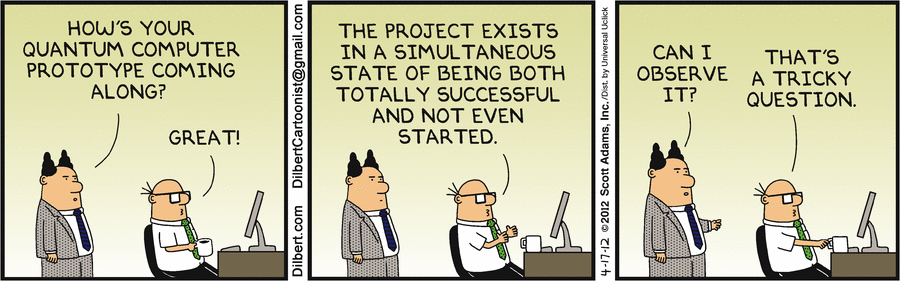
\includegraphics[width=\textwidth]{image/dilbert_quantum_prototype.png}
\end{minipage}



\section{Сферическая блоха. Ой, сфера Блоха}

\section{Вентиль Адамара}

Вентиль Адамара.

\[
H = \frac{1}{\sqrt{2}}\left( \ketbra{0}{0} + \ketbra{0}{1} + \ketbra{1}{0} - \ketbra{1}{1} \right)
\]

\section{Возможные действия}

\section{Алгоритм Дойча}



\[
\Qcircuit @C=1em @R=.7em {
   \lstick{\ket{0}} & \gate{H} & \gate{D} & \gate{H} &  \meter & \qwa
}
\]


\section{Два кубита — два весёлых друга}

\begin{problem}
Алиса посылает Бобу пару кубитов в состоянии\footnote{Конечно, это состояние кубитов, а не Алисы!}
\[
\frac{1}{\sqrt{2}}\ket{00} + \frac{1}{2}\ket{10} + \frac{1}{2}\ket{11}
\]

\begin{enumerate}
  \item Если Боб измерит сразу оба кубита, то каковы будут вероятности каждого состояния?
  \item Боб решил измерить только первый кубит. Каковы вероятности измерить $\ket{0}$ и $\ket{1}$?
  В каких состояниях при этом окажется второй кубит?
  \item Боб решил измерить только второй кубит. Каковы вероятности измерить $\ket{0}$ и $\ket{1}$?
  В каких состояниях при этом окажется первый кубит?
\end{enumerate}

  \begin{sol}
  \end{sol}
\end{problem}

\section{Действия на паре кубитов}


\begin{problem}
Что получит Алиса, если применит действие $H^{\otimes 2}$ к паре кубит
\[
\frac{1}{\sqrt{2}} \ket{00} + \frac{1}{\sqrt{2}}\ket{11}
\]

  \begin{sol}
  \end{sol}
\end{problem}


\begin{problem}
Приведи пример действия $A$ на паре кубит, которое невозможно представить в виде тензорного произведения действий.
То есть невозможно придумать такие однокубитные действия $B$ и $C$, что $A = B \otimes C$.
\begin{sol}
  Например, $CNOT = \ketbra{00}{00} + \ketbra{01}{01} + \ketbra{10}{11} + \ketbra{11}{10}$.
\end{sol}
\end{problem}



\section{Алгоритм Гровера: 2 кубита}

\[
\Qcircuit @C=1em @R=.7em {
   \lstick{\ket{00}} & \gate{H^{\otimes 2}} & \gate{G} & \gate{2\ketbra{++}{++} - I} &  \meter & \qwa
}
\]

\section{Алгоритм Гровера: 3 кубита}

\[
\Qcircuit @C=1em @R=.7em {
   \lstick{\ket{000}} & \gate{H^{\otimes 3}} & \gate{G} & \gate{2\ketbra{+++}{+++} - I} &  \meter & \qwa
   \gategroup{1}{3}{1}{4}{.7em}{--}
}
\]



\section{Алгоритм Саймона: 2 кубита}


\Closesolutionfile{solution_file}

% для гиперссылок на условия
% http://tex.stackexchange.com/questions/45415
\renewenvironment{solution}[1]{%
         % add some glue
         \vskip .5cm plus 2cm minus 0.1cm%
         {\bfseries \hyperlink{problem:#1}{#1.}}%
}%
{%
}%

\section{Решения}
\protect \hypertarget {soln:1.1}{}
\begin{solution}{{1.1}}
  $\P(X=1)=3/5$, $\P(X=2)=3/10$, $\P(X=3)=1/10$, $\E(X)=1.5$
\end{solution}
\protect \hypertarget {soln:1.2}{}
\begin{solution}{{1.2}}
\end{solution}
\protect \hypertarget {soln:1.3}{}
\begin{solution}{{1.3}}
\end{solution}
\protect \hypertarget {soln:1.4}{}
\begin{solution}{{1.4}}
   N 3 4 5

  2/8 3/8 3/8
\end{solution}
\protect \hypertarget {soln:2.1}{}
\protect \hypertarget {soln:2.2}{}
\protect \hypertarget {soln:2.3}{}
\protect \hypertarget {soln:2.4}{}
\protect \hypertarget {soln:3.1}{}
\begin{solution}{{3.1}}
\end{solution}
\protect \hypertarget {soln:3.2}{}
\begin{solution}{{3.2}}
\end{solution}
\protect \hypertarget {soln:10.1}{}
\begin{solution}{{10.1}}
  
\end{solution}
\protect \hypertarget {soln:11.1}{}
\begin{solution}{{11.1}}
  
\end{solution}
\protect \hypertarget {soln:11.2}{}
\begin{solution}{{11.2}}
  Например, $CNOT = \ketbra{00}{00} + \ketbra{01}{01} + \ketbra{10}{11} + \ketbra{11}{10}$.
\end{solution}




\end{document}
